\documentclass[a4paper,11pt]{article}

%%%%%%%%%%%%%%%%%%%%%%%%%%%%%%%%%
%    PACKAGES AND DEFINITIONS   %
%%%%%%%%%%%%%%%%%%%%%%%%%%%%%%%%%
\usepackage{amssymb}
\usepackage{amsmath}
\usepackage{epsfig}
\usepackage{booktabs}
\usepackage{subfig}

\usepackage{fancyhdr}
\usepackage{lastpage}
\usepackage{verbatim}
\usepackage[usenames,dvipsnames]{color}
\usepackage[hyperindex, linktocpage]{hyperref}
\usepackage[english]{babel}
\usepackage{fullpage}
\usepackage{graphicx}

\usepackage[final]{listings}
\usepackage{color}

\lstloadlanguages{[GNU]C++}
\lstset{
    frameround=fttt,
    language=[GNU]C++,
    numbers=left,
    breaklines=true,
    keywordstyle=\color{blue}\bfseries, 
    basicstyle=\ttfamily\color{black},
    numberstyle=\color{black}
}

\usepackage{indentfirst}

\newcommand{\class}{Computer Vision}
\newcommand{\expT}{Object recognition and tracking}
\newcommand{\cand}{Giovanni Fregonese ID 1232107; email: giovanni.fregonese@studenti.unipd.it \\
                   Emilio Olivastri ID 1224048; email: emilio.olivastri@studenti.unipd.it}
\newcommand{\dateD}{June 4th 2020}


\begin{document}

\begin{center}
	\Large
	\begin{center}
		\textsl{Laboratory 6: \expT}\\
		\large
		\hfill\break
		\textsl{\cand}\\
		\dateD
	\end{center}
\end{center}

\subsection*{Activity Goal}

The goal of the laboratory was to develop a program that track the books in the given video.
First we needed to find and match features from target images of the books to the first frame.
The we tracked those features using an optical flow algorithm. 


\subsection*{Lesson Learned}

We found ou that illumination is extremely important: the first book to track, Fundamentals of Deep Learning, was especially diffcult to find in the video.
This was probably due to the fact that the illumation is not uniform and in particular this book is reflecting the light (Figure \ref{fig:book1}). 
The other books were easier to track.

To obtain a robust tracking of the books we employed a function to check whether each tracked feature was inside the rectangle defined by the corners for each book.
This greatly improved the performace of the tracking since the outlines were not influenced by points tracked on other books.

To improve the matching of the templates to the first frame we needed to increase drastically the number of features found on both the templates and the frame.
In the end we settled on 2000 features on the templates and 50000 on the frame, with a discard ratio to discard the outliers of 5.

In the end we obtained this \href{https://youtu.be/u_683hzvI8o}{video}.

The code developed can be found on \href{https://github.com/giotherobot/Lab6_CV}{GitHub}


\begin{figure}[ht]
    \centering
    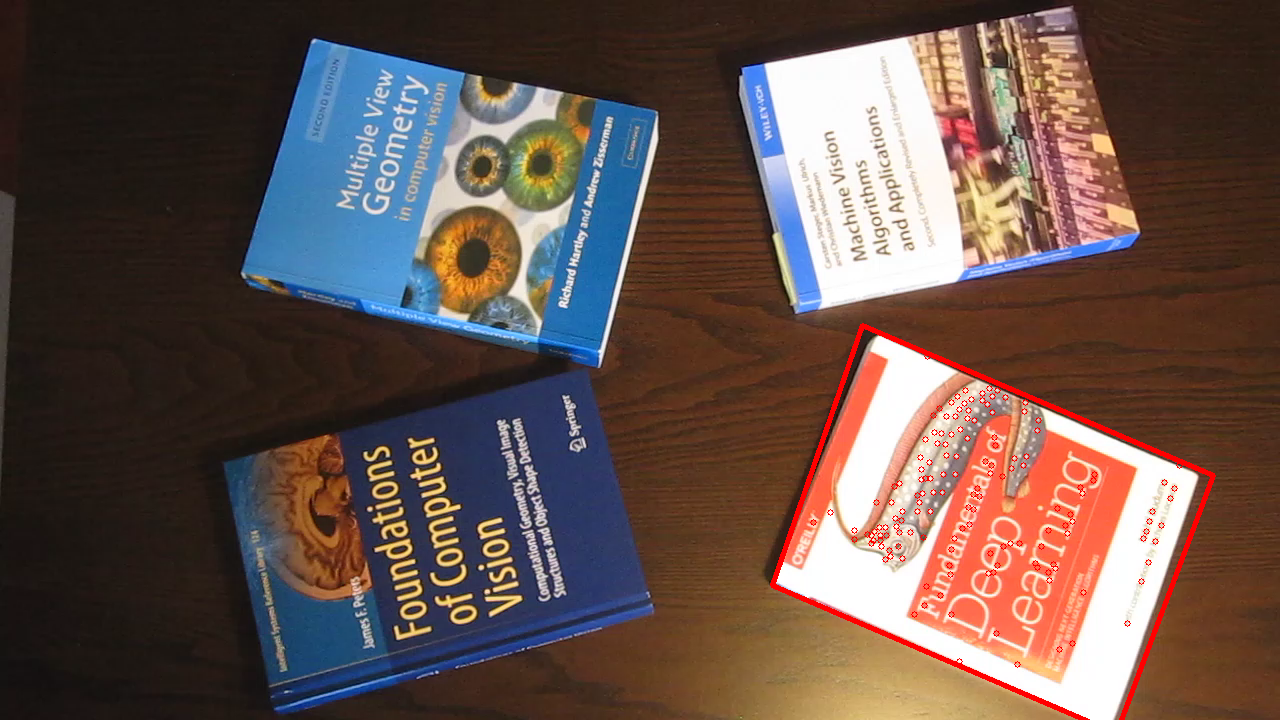
\includegraphics[width=\textwidth]{imgs/TrackedFeatures0.png}
    \caption{Tracked book 1}
    \label{fig:book1}
\end{figure}

\begin{figure}[ht]
    \centering
    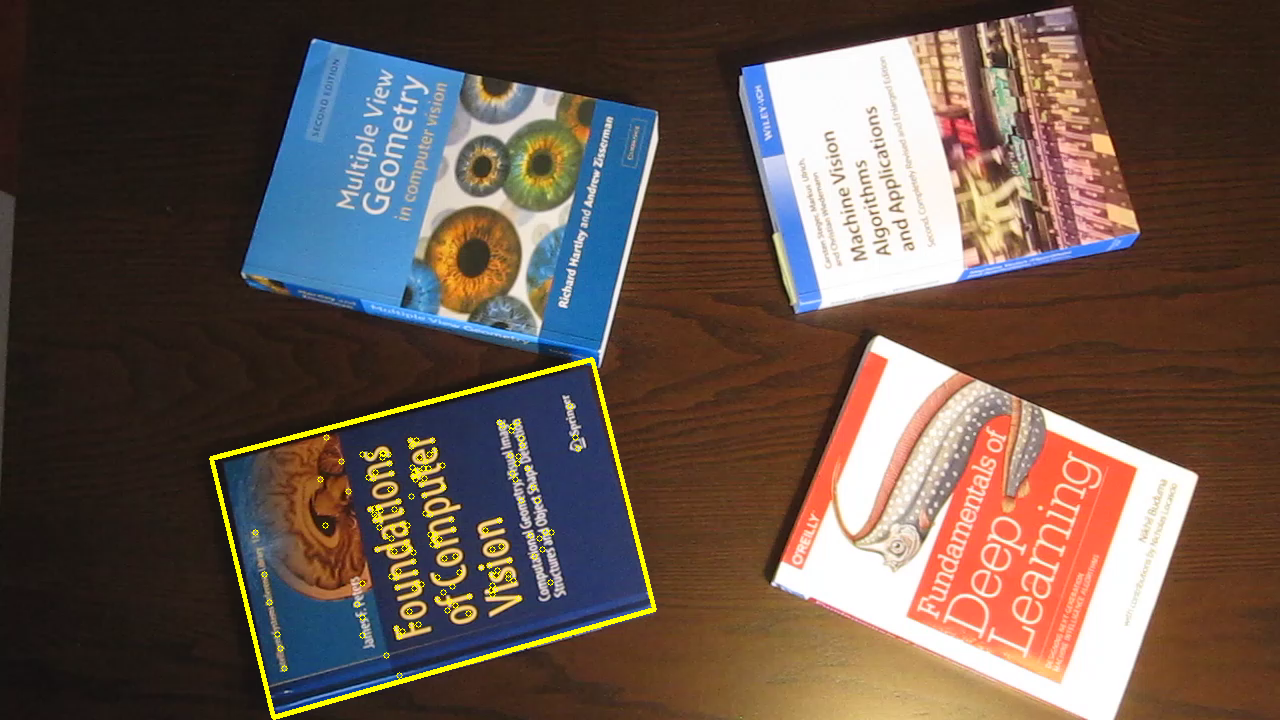
\includegraphics[width=\textwidth]{imgs/TrackedFeatures1.png}
    \caption{Tracked book 2}
    \label{fig:book2}
\end{figure}

\begin{figure}[ht]
    \centering
    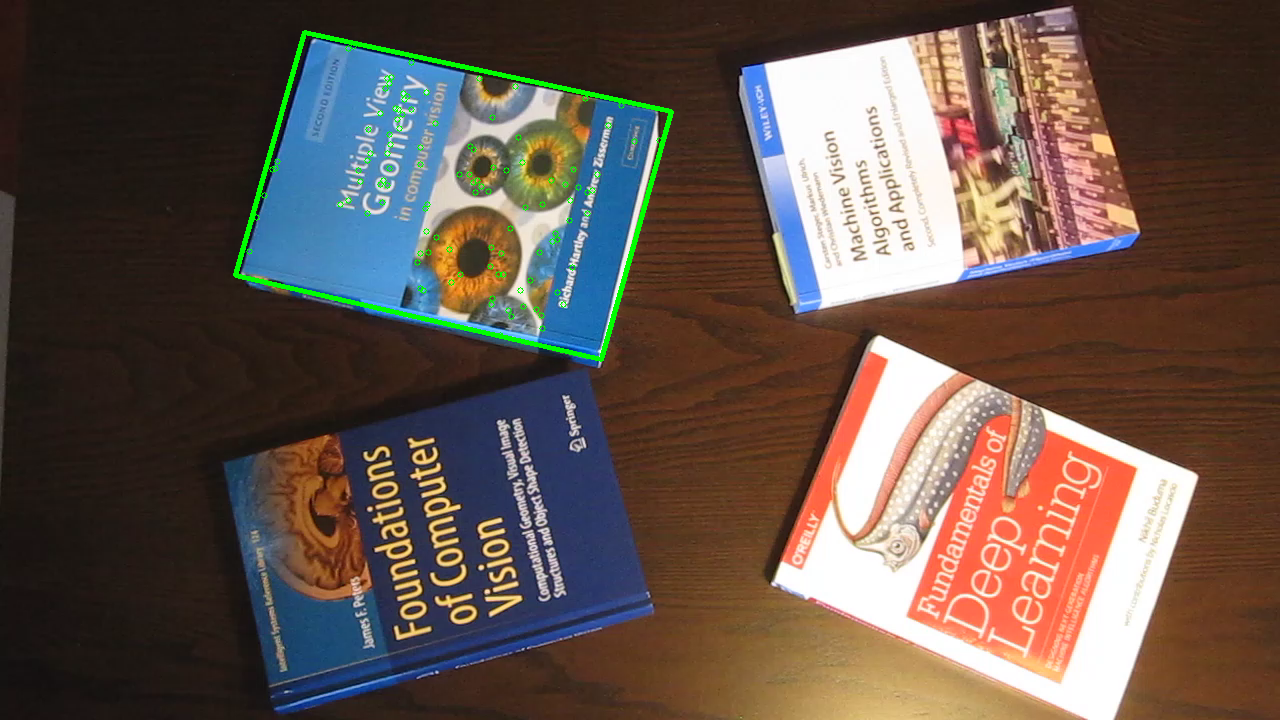
\includegraphics[width=\textwidth]{imgs/TrackedFeatures2.png}
    \caption{Tracked book 3}
    \label{fig:book3}
\end{figure}

\begin{figure}[ht]
    \centering
    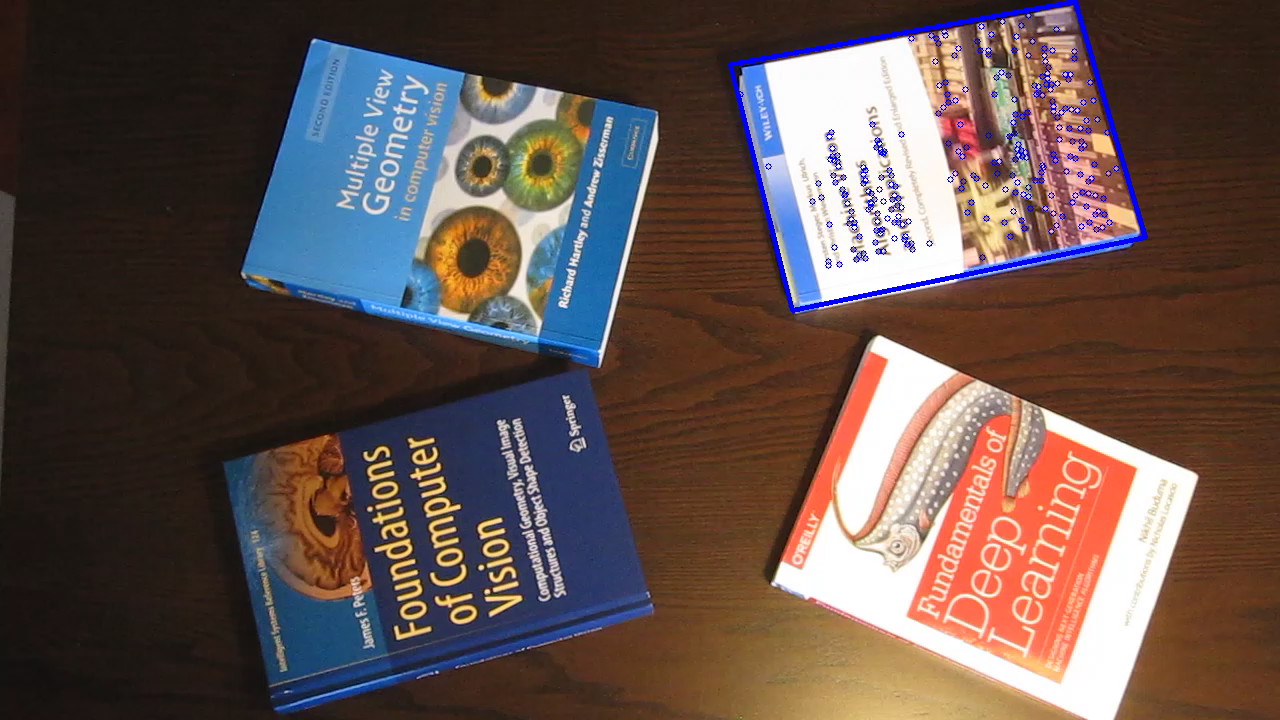
\includegraphics[width=\textwidth]{imgs/TrackedFeatures3.png}
    \caption{Tracked book 4}
    \label{fig:book4}
\end{figure}

\end{document}